% !TeX root = ../main.tex
% !TEX root = ../main.tex
% -*- root: ../main.tex -*-
% -*- program: pdflatex -*-
\chapter{喷注味道鉴别流程}
基于机器学习算法设计喷注味道鉴别分类器需要有三个过程,即训练,验证和测试。训练阶段用一部分样本(训练集)对机器学习模型训练,使模型的鉴别能力不断优化提升;验证过程用一部分样本(验证集,不包含训练集)评估训练阶段获得模型的性能,并根据模型在验证集上的性能更改模型超参数,继续进行训练;测试过程用一部分样本(不能包含训练集,测试集)对经过训练,验证过程后的模型进行测试。整个系统主要由四部分组成:数据获取,数据预处理,特征选择和训练,其流程示意图如图~\ref{fig:model_process}~所示。
\begin{figure}[!htb]
  \centering
  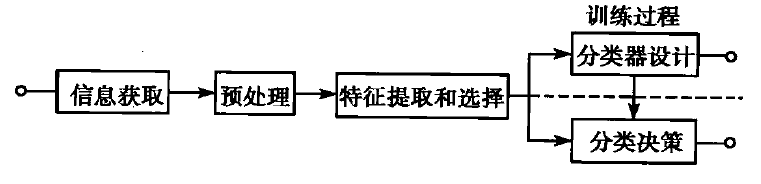
\includegraphics[width=10cm]{chap1/model_process.png}
  \caption{机器学习解决喷注味道鉴别问题流程}
  \label{fig:model_process}
\end{figure}

\section{原始数据获取}
在CEPC实验中,能够被探测装置直接探测到的基本粒子必须满足如下条件:(1).必须是稳定粒子或者有较长的寿命,这样粒子可以在探测器中飞行较长的距离;(2).能够与探测器装置中的物质发生相互作用,因此可以被探测器测量。能够满足上述条件的基本粒子只有有限的几种,常见的有:
$$\gamma,~~ e^{\pm},~~ \mu^{\pm},~~ \pi^{\pm},~~ K^{\pm}, p,~~ \overline{p}.$$
高能物理实验观测到的是上述粒子的响应输出信号,分为时间( TDC )信息和幅度( ADC )信息。CEPC预研阶段,使用Geant4模拟上述信息,将其储存在计算机集群中,以供离线的物理分析。

\section{原始数据预处理}
探测器观测记录的时间信息和幅度信息数据虽然包含了事例的全部可观测信息,但这些信息不能反映事例的”面貌“和性质,不能用来直接作物理分析。将原始数据转化为能够直接反映粒子性质的物理数据过程称为预处理。高能物理的数据预处理包含模拟和重建两个过程。这两个过程在~\cite{zhengzhipeng}中有详细讲解,本文不作介绍。

\section{特征提取和选择}
为了有效地对事例分类识别,需要对预处理后的数据进行筛选和变换,以获得反映事例分类本质特征的物理量,这一过程就是特征提取和选择。特征提取和选择应该有如下三个原则:

(1).有效性,即经过特征提取后的物理量应该能够有效区分信号和本底。

(2).充分性,即提取特征后能够保留事例的完整信息。

(3).具有降维能力,通过特征提取能够有效地减少用它区分信号和本底所需的计算量。

本文用Geant4软件通过蒙特卡洛算法模拟产生CEPC喷注原始数据,并经过模拟和重建过程,获得预处理数据,然后经过特征提取和选择过程,提取事例的63个物理特征。提取特征变量参考~\cite{lcfi}。经过上述过程处理后的数据包含3类:b夸克,c夸克和其他夸克。每类包含210000事例。每个事例包含63个变量。本课题将所有事例分为训练集(400000个事例),3个验证集(每个验证集包含50000个事例)和测试集(80000事例)。

\section{模型训练}
本文使用机器学习的方法获得喷注味道鉴别分类器。采用的算法为神经网络和基于决策树的集成算法。神经网络算法和基于决策树的集成算法将在第三章和第四章作详细介绍。

\section{机器学习分类器的性能度量}
性能度量( performance measure ) 是衡量模型能力的评价标准。在对比不同的模型时,使用不同的性能度量往往会导致不同的评判结果~\cite{zhouzhihua}。本文从精度,信号选择效率,本底排斥率和模型训练时间等方面比较不同模型的性能对比。\\
\subsection{精度}
精度(accuracy)是指样本中被正确分类的事例占事例总数的比例。\\

\subsection{信号效率,误判率}
虽然通过精度可以反映分类器判断事例味道的整体准确度,但对于特殊的任务,比如要求尽量多地将信号事例挑选出来,或者挑出来的信号尽可能是正确的,这时精度就不能作为评判依据,需要使用其他的性能度量。

对于喷注味道鉴别,根据其真实的类别和分类器模型预测的类别组合可将其划分为真正例( True Positive, TP ), 假正例( False Postive, FP ), 假负例( False Negative, FN )和真负例( True Negative, TN )四种情形。四种情形分别为:

真正例:真实类别为信号,预测类别也为信号的事例。

假正例:真实类别为本底,预测类别为信号的事例。

假负例:真实类别为信号,预测类别为本底的事例。

真负例:真实类别为本底,预测类别也本底为的事例。

预测结果的混淆矩阵( confusion matrix )如表~\ref{tbl:confusion_matrix}~所示。
\begin{table}[h]
    \centering
    \caption{\label{tbl:confusion_matrix} 预测结果的混淆矩阵}
    \footnotesize
    \begin{tabular}{|c|c|c|}
        \hline
        %\multirow 纵向合并 \multicolumn横向合并 |c| 两侧添加竖线
        \multirow{2}*{真实情况} & \multicolumn{2}{|c|}{预测结果}\\
        \cline{2-3}
        ~&正例& 反例\\
        \cline{1-3}
        正例& TP(真正例)& FN(假反例)\\
        反例& FP(假正例)& TN(真反例)\\
        \hline
    \end{tabular}
\end{table}

信号效率的定义为:
$$E_{sig} = \frac{TP}{TP+FN}$$

本底排斥率的定义为:
$$E_{bkg} = \frac{TN}{TN+FP}$$

信号效率和本底排斥率是一对矛盾的度量。一般来说,信号效率高时,本底排斥率往往偏低,而本底排斥率高时,信号效率往往偏低。通过训练获得分类器后,可根据不同的判选条件得到分类器不同的信号效率,本底排斥率,然后以信号效率为纵轴,本底排斥率为横轴,绘制$E_{sig}$-$E_{bkg}$曲线,通过$E_{sig}$-$E_{bkg}$曲线,可以对分类器在不同判选条件下的本底排斥率和信号效率有直观的了解。